\section{Wavelet Trees}

\begin{Definition}
  A \defi{wavelet tree}{Wavelet Tree} is a compact datastructure that stores a sequence $S$ and generalizes the operations of a bitvector to an arbitrary alphabet.
  \begin{itemize}
    \item $\proc{Access}(i)$ returns the $i$-th element of the sequence.
    \item $\proc{Rank}_q(i)$ returns the number of occurrences of $q$ in the prefix $S[0..i-1]$.
    \item $\proc{Select}_q(i)$ returns the position of the $i$-th occurrence of $q$ in $S$.
  \end{itemize}

  The root of the wavelet tree stores the whole sequence. Each vertex recursively divides its sequence to its two children. The left child contains the first half of the remaining alphabet, the right child contains the second half of the remaining alphabet. A bitvector in every vertex stores the corresponding child for each element.
\end{Definition}

\begin{Lemma}
  A wavelet tree can be stored in $n\lceil\log\sigma\rceil$ bits space.
\end{Lemma}

\begin{Proof}
  The wavelet tree has height $\lceil\log\sigma\rceil$ and stores $n$ bits on every layer (maybe even less on the last layer). Therefore $n\lceil\log\sigma\rceil$ bits are needed to store the bitvectors. A wavelet tree can be implemented fully via bitvectors and does not need any pointers. This will be demonstrated in more detail below.
\end{Proof}

\begin{Example}
  \label{exp:waveletTree}
  Figure~\ref{fig:waveletTreeExample} shows the wavelet tree for the string "abracadabra". By concatenating the bitvectors in each vertex in level order from left to right, we fully describe the wavelet tree. The bitvector describing this wavelet tree is \texttt{00100010010|00010000|101|0100010}, where the vertical lines show the borders between consecutive vertices. They do not need to be stored, because all layers (except maybe the last layer) contain exactly $n$ bits.
  \begin{figure}[htb]
    \centering
    \def\foo{\vphantom{fy}}
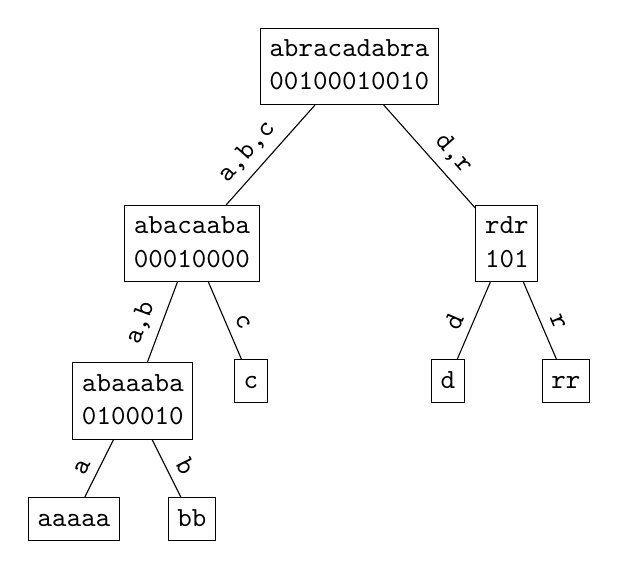
\begin{tikzpicture}[every text node part/.style={align=center}]
  \node[draw] (0) at (0,0) {\texttt{abracadabra}\foo\\\texttt{00100010010}\foo};
  \node[draw] (1) at (-2,-2.25) {\texttt{abacaaba}\foo\\\texttt{00010000}\foo};
  \node[draw] (2) at (-2.75,-4.25) {\texttt{abaaaba}\foo\\\texttt{0100010}\foo};
  \node[draw] (3) at (-1.25,-4) {\texttt{c}\foo};
  \node[draw] (4) at (2,-2.25) {\texttt{rdr}\foo\\\texttt{101}\foo};
  \node[draw] (5) at (1.25,-4) {\texttt{d}\foo};
  \node[draw] (6) at (-3.5,-5.75) {\texttt{aaaaa}\foo};
  \node[draw] (7) at (-2,-5.75) {\texttt{bb}\foo};
  \node[draw] (8) at (2.75,-4) {\texttt{rr}\foo};

  \draw (0) -- (1) node [above,sloped,pos=0.6] {\texttt{a,b,c}};
  \draw (1) -- (2) node [above,sloped,pos=0.6] {\texttt{a,b}};
  \draw (1) -- (3) node [above,sloped,pos=0.6] {\texttt{c}};
  \draw (0) -- (4) node [above,sloped,pos=0.6] {\texttt{d,r}};
  \draw (4) -- (5) node [above,sloped,pos=0.6] {\texttt{d}};
  \draw (4) -- (8) node [above,sloped,pos=0.6] {\texttt{r}};
  \draw (2) -- (6) node [above,sloped,pos=0.6] {\texttt{a}};
  \draw (2) -- (7) node [above,sloped,pos=0.6] {\texttt{b}};
\end{tikzpicture}

    \caption{The wavelet tree for the string "abracadabra".}
    \label{fig:waveletTreeExample}
  \end{figure}
\end{Example}

When storing the wavelet tree in a single bitvector $B$ as in Example~\ref{exp:waveletTree}, each vertex can be described by two indices giving the position of the bitvector of the vertex in $B$. For example the root corresponds to the pair $[0,n-1]$. Algorithm~\ref{alg:waveletTreeLevel} shows how to get the level of a vertex $v$ of the wavelet tree. This just uses the fact, that every level contains $n$ bits. Algorithm~\ref{alg:waveletTreeSize} calculates the length of the string stored in the given vertex. Algorithm~\ref{alg:waveletTreeLeftChild} and Algorithm~\ref{alg:waveletTreeRightChild} return the indices for the left and the right child of the given vertex. Assuming that we can execute the rank queries in constant time (Theorem~\ref{thm:bitvectorRank}), they both run in constant time. It is also possible to implement a \proc{Parent}-function, but this needs additional information, such as whether the current vertex is a left or a right child of its parent.

\begin{algorithm}[htb]
  \begin{codebox}
    \Procname{$\proc{Level}(v=[l,r])$}
    \li \Return $\left\lceil \frac{l}{n} \right\rceil$
  \end{codebox}
  \caption{Returns the level of a vertex of the wavelet tree.}
  \label{alg:waveletTreeLevel}
\end{algorithm}

\begin{algorithm}[htb]
  \begin{codebox}
    \Procname{$\proc{Size}(v=[l,r])$}
    \li \Return $r - l + 1$
  \end{codebox}
  \caption{Returns the number of elements stored in a vertex of the wavelet tree.}
  \label{alg:waveletTreeSize}
\end{algorithm}

\begin{algorithm}[htb]
  \begin{codebox}
    \Procname{$\proc{Left-Child}(v=[l,r])$}
    \li $l' \gets l + n$
    \li $r' \gets l' + \proc{Size}(v) - (\proc{Rank}(r + 1) - \proc{Rank}(l)) - 1$
    \li \Return $[l',r']$
  \end{codebox}
  \caption{Returns the left child of a vertex of the wavelet tree.}
  \label{alg:waveletTreeLeftChild}
\end{algorithm}

\begin{algorithm}[htb]
  \begin{codebox}
    \Procname{$\proc{Right-Child}(v=[l,r])$}
    \li $r' \gets r + n$
    \li $l' \gets r' - (\proc{Rank}(r + 1) - \proc{Rank}(l) - 1)$
    \li \Return $[l',r']$
  \end{codebox}
  \caption{Returns the right child of a vertex of the wavelet tree.}
  \label{alg:waveletTreeRightChild}
\end{algorithm}

\begin{Theorem}
  \label{thm:waveletTreeAceess}
  The $\proc{Access}(i)$-operation can be implemented in $\mathcal{O}(\log \sigma)$.
\end{Theorem}

\begin{Proof}
  To access the $i$-th element we check the $i$-th position in the root-bitvector. If it is $0$, the element is stored in the left child and the new index there is $i - \proc{Rank}_1(i)$. If it is $1$, the element is in the right child and the new index there is $i - \proc{Rank}_0(i)$.

  This can be done in $\mathcal{O}(\log\sigma)$, because the wavelet tree has a height of $\log\sigma$ and the rank queries can be done in constant time on bitvectors.
\end{Proof}

\begin{Theorem}
  \label{thm:waveletTreeRank}
  The $\proc{Rank}_q(i)$-operation can be implemented in $\mathcal{O}(\log \sigma)$.
\end{Theorem}

\begin{Proof}
  $\proc{Rank}_q(i)$-queries can be answered the same way as $\proc{Access}(i)$-queries. The $\proc{Access}(i)$-query descents into the leaf containing all $q$ symbols with some modified index $i'$. The rank is the number of elements before $i'$, so $i'-1$. Since no additional work needs to be done, the runtime is in $\mathcal{O}(\log\sigma)$.
\end{Proof}

\begin{Theorem}
  \label{thm:waveletTreeSelect}
  The $\proc{Select}_q(i)$-operation can be implemented in $\mathcal{O}(\log \sigma)$.
\end{Theorem}

\begin{Proof}
  % TODO (pjungeblut): This uses the fact, that select-queries can be done in
  %                    constant time on bitvectors. This is not yet proven in
  %                    this document. If added, also remove parentheses from
  %                    the last sentence in the following paragraph.
  For a $\proc{Select}_q(i)$-query we start in the leave corresponding to symbol $q$ at position $i$. This can be found the same way as in the $\proc{Access}$-operation. Now we recursively process the parents until reaching the root. If the current vertex is a left child, the new position is the position of the $i$-th $0$ in the parent bitvector. If it is a right child, the new position is the position of the $i$-th $1$ in the parent bitvector. This needs $\proc{Select}$-queries on bitvectors, which can be done in constant time (not part of this document yet).
\end{Proof}

Another commonly used method on wavelet trees is \proc{Expand} given as pseudocode in Algorithm~\ref{alg:waveletTreeExpand}. If we are given an interval $[i,j]$ in the bitvector of some node $v=[l,r]$, \proc{Expand} splits this interval into two intervals $[i_l,j_l]$ and $[i_r,j_r]$ of the left and right child.

\begin{algorithm}[htb]
  \begin{codebox}
    \Procname{$\proc{Expand}(v = [l,r], [i,j])$}
    \li $i_l \gets \proc{Rank}_0(i)$
    \li $j_l \gets \proc{Rank}_0(j)$
    \li $i_r \gets \proc{Rank}_1(i)$
    \li $j_r \gets \proc{Rank}_1(j)$
    \li \Return $\langle [i_l,r_l], [i_r,j_r] \rangle$
  \end{codebox}
  \caption{Expands a range $[i,j]$ of node $v$ into two child ranges.}
  \label{alg:waveletTreeExpand}
\end{algorithm}

\begin{Example}
  Let $A$ be an integer array of size $n$. We want to answer range median queries with an $\mathcal{O}(n\log n)$ datastructure in time $\mathcal{O}(\log n)$. Here the median of a range $A[i,j]$ is defined as the $\lceil \frac{j - i + 1}{2} \rceil$-th smallest element in $A[i,j]$.

  The solution is given in Algorithm~\ref{alg:rangeMedianQuery}. It uses an integer wavelet tree and \proc{Expand} to find the median.
  \begin{algorithm}[htb]
    \begin{codebox}
      \Procname{$\proc{Range-Median-Query}([i,j])$}
      \li $\id{median} \gets \frac{j - i + 1}{2}$
      \li $v \gets [0,n-1]$ \>\>\>\>\>\>\>\>\Comment Root of the wavelet tree.
      \li $\id{range} \gets [i,j]$
      \li \While not $\proc{Is-Leaf}(v)$
          \Do
      \li   $\id{childRanges} \gets \proc{Expand}(v, \id{range})$
      \li   \If \proc{Size}(\id{childRanges}[0]) > \id{median}
            \Then
      \li     $v \gets \proc{Left-Child}(v)$
      \li     $\id{range} \gets \id{childRanges}[0]$
      \li   \Else
      \li     $v \gets \proc{Right-Child}(v)$
      \li     $\id{range} \gets \id{childRanges}[1]$
            \End
          \End
      \li \Return $\proc{symbol}(v)$
    \end{codebox}
    \caption{Range median queries in an integer array.}
    \label{alg:rangeMedianQuery}
  \end{algorithm}
\end{Example}
